\documentclass[tikz,border=8pt]{standalone}
% Shared look for every TikZ diagram. Load with % Shared look for every TikZ diagram. Load with % Shared look for every TikZ diagram. Load with \input{../../tools/tikz-style.tex}
\usepackage[T1]{fontenc}
\usepackage{lmodern}
\renewcommand{\sfdefault}{lmr}  % diagrams use the same serif as the text
\usetikzlibrary{arrows.meta, positioning, shapes.geometric, calc, fit, backgrounds}
\definecolor{cblue}{HTML}{4C78A8}
\definecolor{corange}{HTML}{F58518}
\definecolor{cgreen}{HTML}{54A24B}
\definecolor{cred}{HTML}{E45756}
\definecolor{cpurple}{HTML}{B279A2}
\definecolor{cgrey}{HTML}{6B6B6B}
\tikzset{
  every picture/.style={font=\sffamily, line width=1.2pt},
  box/.style={draw=#1, fill=#1!12, rounded corners=4pt, align=center, inner sep=7pt, minimum height=1.1cm},
  box/.default=cgrey,
  arrow/.style={-{Stealth[length=3mm]}, draw=cgrey, line width=1.4pt},
  title/.style={font=\sffamily\bfseries\Large},
  note/.style={font=\sffamily\small, text=cgrey, align=center},
}
\AtBeginDocument{\hyphenpenalty=10000 \exhyphenpenalty=10000}

\usepackage[T1]{fontenc}
\usepackage{lmodern}
\renewcommand{\sfdefault}{lmr}  % diagrams use the same serif as the text
\usetikzlibrary{arrows.meta, positioning, shapes.geometric, calc, fit, backgrounds}
\definecolor{cblue}{HTML}{4C78A8}
\definecolor{corange}{HTML}{F58518}
\definecolor{cgreen}{HTML}{54A24B}
\definecolor{cred}{HTML}{E45756}
\definecolor{cpurple}{HTML}{B279A2}
\definecolor{cgrey}{HTML}{6B6B6B}
\tikzset{
  every picture/.style={font=\sffamily, line width=1.2pt},
  box/.style={draw=#1, fill=#1!12, rounded corners=4pt, align=center, inner sep=7pt, minimum height=1.1cm},
  box/.default=cgrey,
  arrow/.style={-{Stealth[length=3mm]}, draw=cgrey, line width=1.4pt},
  title/.style={font=\sffamily\bfseries\Large},
  note/.style={font=\sffamily\small, text=cgrey, align=center},
}
\AtBeginDocument{\hyphenpenalty=10000 \exhyphenpenalty=10000}

\usepackage[T1]{fontenc}
\usepackage{lmodern}
\renewcommand{\sfdefault}{lmr}  % diagrams use the same serif as the text
\usetikzlibrary{arrows.meta, positioning, shapes.geometric, calc, fit, backgrounds}
\definecolor{cblue}{HTML}{4C78A8}
\definecolor{corange}{HTML}{F58518}
\definecolor{cgreen}{HTML}{54A24B}
\definecolor{cred}{HTML}{E45756}
\definecolor{cpurple}{HTML}{B279A2}
\definecolor{cgrey}{HTML}{6B6B6B}
\tikzset{
  every picture/.style={font=\sffamily, line width=1.2pt},
  box/.style={draw=#1, fill=#1!12, rounded corners=4pt, align=center, inner sep=7pt, minimum height=1.1cm},
  box/.default=cgrey,
  arrow/.style={-{Stealth[length=3mm]}, draw=cgrey, line width=1.4pt},
  title/.style={font=\sffamily\bfseries\Large},
  note/.style={font=\sffamily\small, text=cgrey, align=center},
}
\AtBeginDocument{\hyphenpenalty=10000 \exhyphenpenalty=10000}

\begin{document}
% One chain-rule factor on the five winning matches of the cricket example (query: toss lost, Mumbai, sunny).
% Left: the exact factor P(toss lost | Mumbai, sunny, win) can only use the wins played in Mumbai in sunny weather: 1 match.
% Right: the naive factor P(toss lost | win) uses all 5 wins.
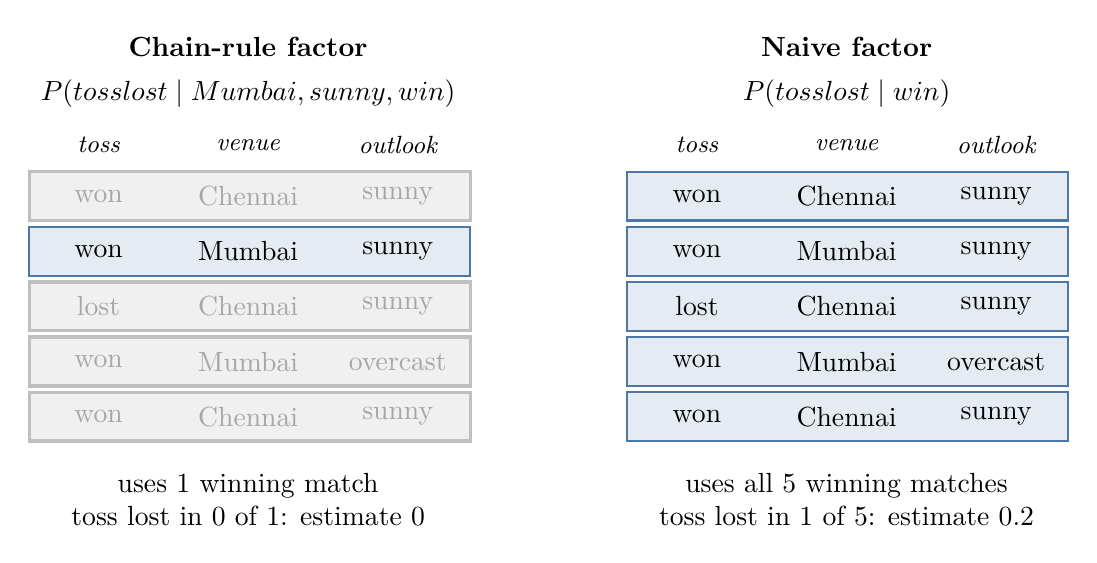
\begin{tikzpicture}[row/.style={minimum height=0.62cm, minimum width=5.6cm, inner sep=0pt, anchor=west}]
  \foreach \xs/\ttl/\sub in {0/{Chain-rule factor}/{$P(\text{toss lost} \mid \text{Mumbai}, \text{sunny}, \text{win})$},
                             7.6/{Naive factor}/{$P(\text{toss lost} \mid \text{win})$}} {
    \begin{scope}[xshift=\xs cm]
      \node[font=\bfseries] at (2.8,1.55) {\ttl};
      \node at (2.8,0.95) {\sub};
      \node[font=\small\itshape] at (0.9,0.3) {toss}; \node[font=\small\itshape] at (2.8,0.3) {venue}; \node[font=\small\itshape] at (4.7,0.3) {outlook};
    \end{scope}
  }
  \foreach \i/\t/\v/\o/\l/\r in {1/won/Chennai/sunny/0/1, 2/won/Mumbai/sunny/1/1, 3/lost/Chennai/sunny/0/1, 4/won/Mumbai/overcast/0/1, 5/won/Chennai/sunny/0/1} {
    \foreach \xs/\on in {0/\l, 7.6/\r} {
      \begin{scope}[xshift=\xs cm, yshift=-\i*0.7cm+0.35cm]
        \ifnum\on=1 \node[row, fill=cblue!15, draw=cblue, thick] at (0,0) {}; \else \node[row, fill=black!6, draw=black!25] at (0,0) {}; \fi
        \ifnum\on=1 \def\c{black}\else\def\c{black!35}\fi
        \node[text=\c] at (0.9,0) {\t}; \node[text=\c] at (2.8,0) {\v}; \node[text=\c] at (4.7,0) {\o};
      \end{scope}
    }
  }
  \node[align=center] at (2.8,-4.2) {uses 1 winning match\\ toss lost in 0 of 1: estimate $0$};
  \node[align=center] at (10.4,-4.2) {uses all 5 winning matches\\ toss lost in 1 of 5: estimate $0.2$};
\end{tikzpicture}
\end{document}
